\section{System organization}

This practical work includes 2 files:
\begin{enumerate}
    \item \textbf{client.c:}
        \begin{itemize}
            \item Open listening Socket
            \item Reads a text file
            \item Sends the file's data to the Server
        \end{itemize}
    \item \textbf{server.c:} 
        \begin{itemize}
            \item Open listening Socket
            \item Receives the data sent by the Client
            \item Saves the data to a new text file
        \end{itemize}
\end{enumerate}
The process\cite{roxtomar2021filetransfer} is demonstrated in Figure \ref{fig:sys-org}.

\begin{figure}
    \centering
    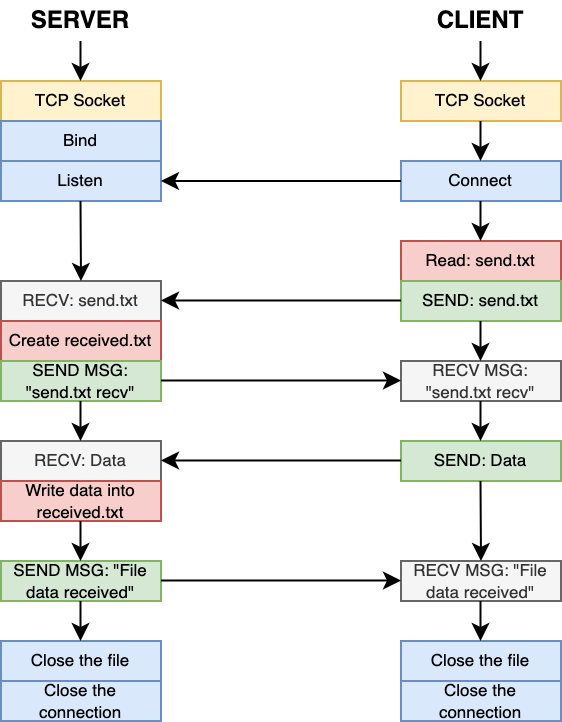
\includegraphics[width=0.9\linewidth]{attachments/system-organization.png}
    \caption{Overall procedure for the TCP file transfer}
    \label{fig:sys-org}
\end{figure}

\subsection{Server Setup}

\begin{itemize}
    \item Initializes a TCP socket.
    \item Binds the socket to an IP address and port (in this case localhost and port 8080).
    \item Listens for incoming client connections.
\end{itemize}

\subsection{Client Setup}

\begin{itemize}
    \item Initializes a TCP socket.
    \item Connects to the server's IP address and port (in this case localhost and port 8080).
\end{itemize}

\subsection{File Transfer Initiation}

\begin{itemize}
    \item The client reads the file \verb|send.txt|.
    \item The client sends the file to the server.
    \item The server receives the filename \verb|send.txt| and creates a new file \verb|received.txt| to store the incoming data.
\end{itemize}

\subsection{Confirmation and Data Transfer}

\begin{itemize}
    \item The server sends a confirmation message back to the client, indicating that the \verb|send.txt| file has been received.
    \item The client starts sending the data to the server.
    \item The server receives the data and writes it into \verb|received.txt|.
\end{itemize}

\subsection{Transfer Completion}

\begin{itemize}
    \item Once the file data is fully transferred, the server sends a message "File data received" to the client.
    \item The client then closes the connection, completing the file transfer process.
\end{itemize}